\chapter{Analysis}

In this section we take a deeper look into the data, the process of augmenting the data, the experiment, and the results. Our partner has provided a small sample of 1000 labeled data points. This data was manually labeled by an annotator. The data consists of a merchant name, merchant website (url), merchant category, and merchant tag as shown in Table \ref{tab:data_point}. 


\begin{table}[h]
\begin{tabular}{|l|l|l|l|}
\hline
merchant name            & merchant url            & merchant category & merchant tags           \\ \hline
State Hospital & http://hospital.com/ & Health   & '\{"Clinic"\}' \\ \hline
\end{tabular}
\caption{This is an example of a single data point.}
\label{tab:data_point}
\end{table}


The current process consists of giving the merchant url to an annotator and the annotator then views the website and either can instantly  provide a label and tags for the website or in some cases may need to browse further into the website (by viewing sibling pages such as the 'About Us' sections or product pages) to get an idea of how the website should be classified. 

The merchant tags are ordered by relevance, with the first tag in the list being the most general and the final being the most specific. An example of the tag hierarchy is show in Table. \ref{tab:tags} where we can see that this sample consists of data from various categories all contained within the 'Eco' side tag grouping.


\begin{table}[h]
\begin{tabular}{|l|l|l|l|l|}
\hline
Category       & Level 1                     & Level 2                       & Level 3      & Side Tag \\ \hline
Travel         & Local Transport             & Micro-mobility                & Bike Sharing & Eco      \\ \hline
               &                             & Public Transport              &              & Eco      \\ \hline
Fashion        & Clothing - Other            & Second Hand                   &              & Eco      \\ \hline
Car            & Charging Station            &                               &              & Eco      \\ \hline
               & Car Sharing                 &                               &              & Eco      \\ \hline
\end{tabular}
\caption{This is an example of how the tags use different levels.}
\label{tab:tags}
\end{table}


Similarly to the annotator our goal is to automate the navigation, collection/storing process, and classification of the website. This pipeline speeds up the browsing process and can allow the annotator to spend much less time annotating and require the annotator to only anotate data expected to drastically improve the classifier.

\subsection{Data}

The initial 1000 data points we received were essentially just labels. The labels needed the text from the websites that the annotator viewed to begin the classifing process. Out of these initial data points 179 contained links that could not be accessed or links that provided no text data that could be scraped. Out of the remaining 821 data points 274 of them were in English. 

It is important for us to have the data in Englsih as it allows us to exploit stop words when using the scikit-learn TF-IDF Vectorizer to construct our dataset. Stop words are words like “and”, “the”, “him”, which are presumed to be uninformative in representing the content of a text, and which may be removed to avoid them being construed as signal for prediction (\cite{sklearn62feature}).

\begin{figure}[!h]
  \centering
  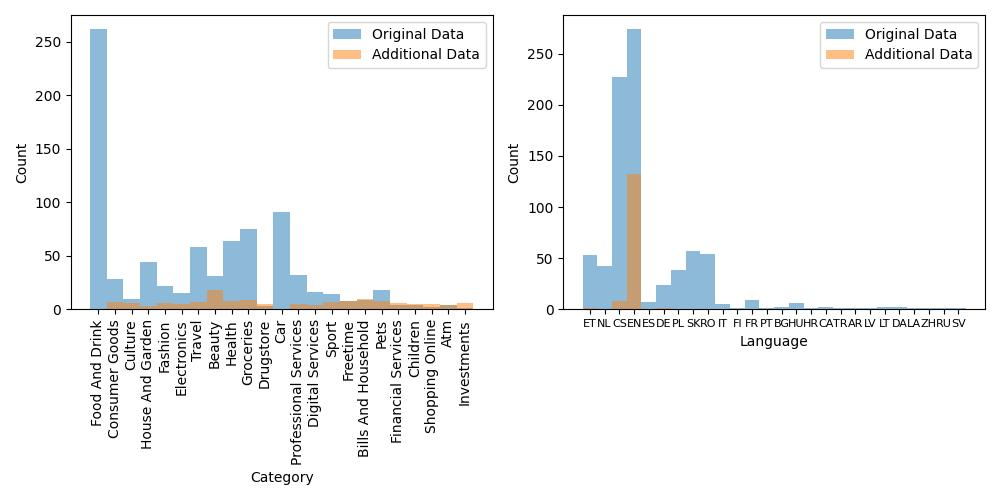
\includegraphics[width=\textwidth]{../img/data_overview.jpg}
  \caption{The histograms for the original data provided.}
  \label{fig:data_histogram}
\end{figure}


\section{The Data}
The data we are working with is a 


\section{Experiments}

\section{Results and Analysis}
